% Copyright (C) 2013 Thomas L. Kula
% All Rights Reserved
%
% See the file LICENSE for license terms.
\documentclass[12pt]{article}
\usepackage{graphicx}
\usepackage{rotating}
\usepackage{fix-cm}
\usepackage{multirow}
\setlength{\paperwidth}{5.5in}
\setlength{\paperheight}{8.5in}
\setlength{\textheight}{7.45in}
\setlength{\topmargin}{-1.0in}
\setlength{\oddsidemargin}{-0.5in}
\setlength{\evensidemargin}{-0.5in}
\setlength{\textwidth}{4.0in}
\setlength{\parindent}{0in}
\setlength{\parskip}{3mm}
\usepackage[print]{booklet} \nofiles
\source{\magstep0}{5.5in}{8.5in}
\target{\magstep0}{11in}{8.5in}
\setpdftargetpages
\pagestyle{empty}
\begin{document}


\begin{center}
{\fontsize{36}{48}\selectfont \textsc{Haiku a Day }}
\end{center}

\vspace*{3.5cm}

{\fontsize{20}{40}\selectfont 

Oh stupid printer

You're always jamming on me

Please just work smoothly

}

\vspace*{5.0cm}
\begin{center}
{\large{Issue 92: February 2013}} \\[5mm]
{\fontsize{8}{8}\selectfont  \textsc{ St. Joshua Norton Press }} \\[1mm]
{\fontsize{6}{6}\selectfont Mathom House by the Cloisters \textbar The People's Republic of Ames }
\end{center}


\newpage

For the past week, the local ice cream truck has been driving around the neighborhood,
playing its music. I love that guy's optimism.

--- Thomas

http://kula.tproa.net/had/ \\
kula@tproa.net

Download this and previous HADs at the website, so you can
print out your own (DIY, yeah!) or if you want me to send
you one, send me your address, and maybe a stamp if you
are feeling nice. Or send me something you've made ---
trades always appreciated, postcards are nice too.

\vfill

\newpage

1 February 2013

Closet victory! \\
Doorknob broken, defeated \\
A door now opens

2 February 2013

Sweet vermouth, rocks, twist \\
Phil comes out day after day \\
Watch that first step --- bing!

3 February 2013

On the door a badge \\
Shows the apartment number \\
This is what's within

4 February 2013

A beacon shines bright \\
Yelling 'Doughnuts' in the night \\
Welcome sign in dark times

5 February 2013

Not all can be whole \\
Sometimes you need broken glass \\
To make a mural

6 February 2013

There is a limit \\
To how much I can handle \\
Then I need a nap

7 February 2013

A dusty cupboard \\
With cans you'll never open --- \\
Just go to the store

\newpage

8 February 2013

Closing door, stand clear \\
Your back pack is delaying \\
Just get it inside

9 February 2013

Wake up with grumpy \\
Walk to the corner, coffee \\
The world is good now

10 February 2013

A theater dark \\
Blinds us with jazz from the stage \\
Weighty history

11 February 2013

Not to big or small \\
A medium medium \\
Gets the spirits right

12 February 2013

In situating \\
You must get just the right snug \\
Too much is too bad

13 February 2013

Infinite rainbow \\
A spectrum mostly unseen \\
But very useful

14 February 2013

To the Post Office \\
There is mailing to be done \\
Stamps to be purchased

\newpage

15 February 2013

Sometimes adventure \\
Just means tomato soup and \\
Grilled cheese sandwiches

16 February 2013

Following the bus \\
See that it's the one I need; \\
Wait for the next one

17 February 2013

A cooking mix-up \\
Is a chance to improvise \\
Which turned out ok

18 February 2013

A sword hanging high \\
Arboreal, a branch swings \\
Creaking in the breeze

19 February 2013

Two ships, forever \\
Stuck in a sea of velvet \\
Sail my living room

20 February 2013

Temptation abounds: \\
A packing tape dispenser --- \\
Taping ALL the things!

21 February 2013

Grabbing a sandwich \\
A lack of chips counfounding \\
Almonds it is, then

\newpage

22 February 2013

Find the replacement \\
For an irreplaceable \\
Leads to frustration

23 February 2013

The horizon shrinks \\
Distances once short, lengthen \\
Here in the city

24 February 2013

A simple labor \\
Folding all of the laundry \\
Confounded by naps

25 February 2013

A dozen is twelve \\
Randomly, I wonder why \\
Latin is to blame

26 February 2013

Boil long enough \\
And you make a nice syrup; \\
To long, it's carbon

27 February 2013

In the neighborhood \\
Mr. Rogers may be gone \\
But his deeds live on

28 February 2013

In squeezing olives \\
There's a wonderful oil; \\
It's good on salads


\newpage

\begin{center}
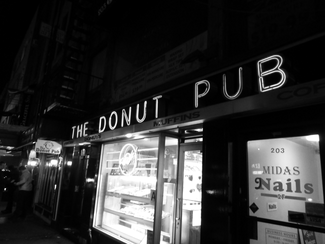
\includegraphics[width=325pt]{doughnut.png}
The Donut Pub \\
9 February 2013 \\
{\tt kula.tproa.net/photos/2013/20130209-subway-shuffle }
\end{center}

\newpage

\thispagestyle{empty}
\vspace*{12cm}
\begin{sideways}
\Large{St. Joshua Norton Press}
\end{sideways}
\begin{sideways}
\Large{PO Box 250138}
\end{sideways}
\begin{sideways}
\Large{New York NY 10025}
\end{sideways}


\end{document}


